\section{Motivation}
\label{sec:motivation}

We present a to-do list application to showcase the
functionality of \dsl{}.

\subsection{Running Example}

Our application has two screens: a main screen and a menu screen. The main screen contains a navigation bar and three items. An overview of the application is given in Figure~\ref{fig:appOverview}. These screenshots are captured from the application built by combining \dsl{} with \texttt{gloss}.

\begin{figure}[!htbp]
\centering
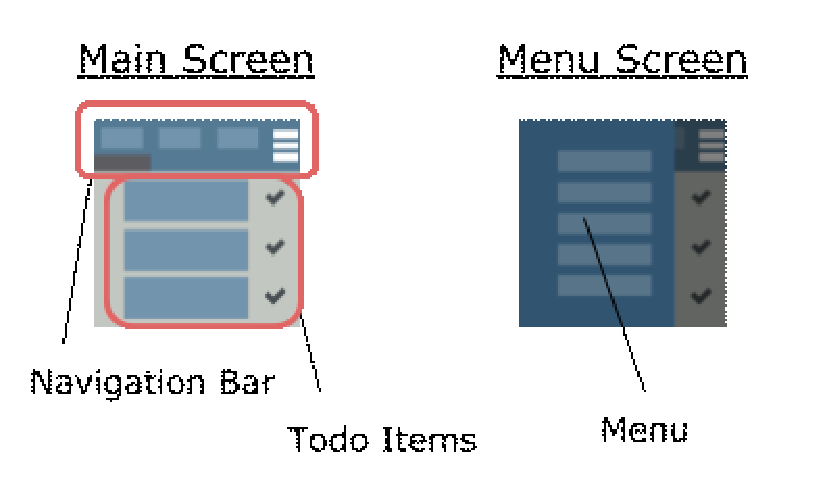
\includegraphics[width=\figscale\textwidth]{pictures/app_overview}
\caption{Overview of the to-do list application.}
\label{fig:appOverview}
\end{figure}

In this application, various user actions are accompanied with an animation.
We list these actions below. Some animations are shown in Figure~\ref{fig:animExamples}.
\begin{itemize}
\item The user marks items as \emph{(not) done} by clicking them. The
checkmark icon changes shape and color to display its status change.
\item The user filters items by their status with the navigation bar
buttons. The leftmost shows all items, the middle shows all done items, and
the rightmost shows all to-do items. The navigation bar underline and to-do
items itself change shape to indicate the new selection.
\item The menu screen shows/hides itself after clicking the hamburger icon. The
menu expands inward from the left, to indicate the application state change.
\end{itemize}

\begin{figure}[!htbp]
\centering

\begin{subfigure}[h]{\textwidth}
\centering
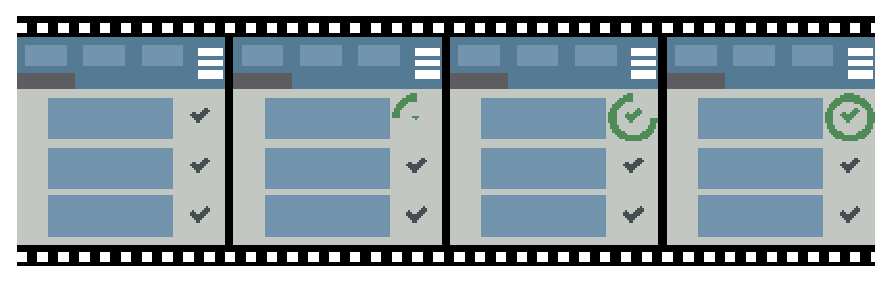
\includegraphics[width=\figscale\textwidth]{pictures/completeIconCheckFig}
\caption{\hs{markAsDone}: the checkmark changes shape and color.}
\label{fig:completeIconCheck}
\end{subfigure}

\begin{subfigure}[h]{\textwidth}
\centering
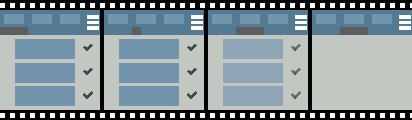
\includegraphics[width=\figscale\textwidth]{pictures/onlyDoneFig}
\caption{\hs{onlyDone}: the to-do items fade out and the navbar underline changes.}
\label{fig:onlyDoneFig}
\end{subfigure}

\begin{subfigure}[h]{\textwidth}
\centering
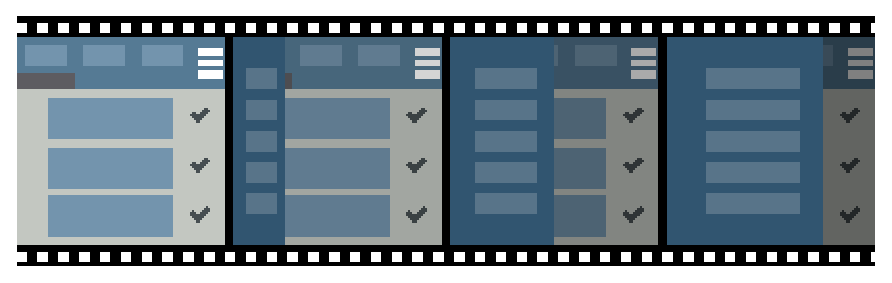
\includegraphics[width=\figscale\textwidth]{pictures/menuIntroFig}
\caption{\hs{menuIntro}: the menu appears while the background fades out.}
\label{fig:menuIntroFig}
\end{subfigure}

\caption{Micro-Animations in the to-do list application.}
\label{fig:animExamples}
\end{figure}

\subsection{Composing Animations}

Animations are built in compositional fashion. When creating an animation, we decompose it into smaller elements. For example, the \hs{menuIntro} animation both introduces the menu screen and fades out the background. Thus, it is composed of two basic animations \hs{menuSlideIn} and \hs{appFadeOut} in parallel. The next sections explain how to construct such basic and composed animations.

\subsubsection{Basic Animations}

Basic animations change the property of an element over a period of time.
The \hs{linearTo} function has three inputs: a lens targeting the property, the duration,
and the target value for this property. This results in a linear change from
the current value to its target, hence the name. The duration is specified
with \hs{For} while the target value is specified with \hs{To}.

\paragraph{Note on Lenses} We use lens notation \texttt{x . y . z} to
target \texttt{z} inside a nested structure \hs{{ x: { y: { z:
T } } }}. This type of lenses was conceived by van Laarhoven
\cite{vlLenses}, and later packaged into
various Haskell libraries, such as
\texttt{lens}\footnote{\url{https://hackage.haskell.org/package/lens}}.

To animate the navigation bar underline, we reduce the width of the
leftmost underline for 0.25 seconds and increase the width of
the middle underline for 0.25 seconds. These animations are expressed in
respectively \hs{line1Out} and \hs{line2In} below, and shown visually in
Figure~\ref{fig:basic}.

\begin{spec}
line1Out = linearTo (navbar . underline1 . width) (For 0.25) (To 0)
line2In = linearTo (navbar . underline2 . width) (For 0.25) (To 28)
\end{spec}

The \hs{menuSlideIn} and \hs{appFadeOut} animations are other examples. For the
former, we increase the width of the menu over a duration of 0.5 seconds, and
for the latter we increase the alpha value of the obscuring box over a duration
of 0.5 seconds. These animations are shown visually in Figure~\ref{fig:basic}.

\begin{spec}
menuSlideIn = linearTo (menu . width) (For 0.5) (To 75)
appFadeOut = linearTo (obscuringBox . alpha) (For 0.5) (To 0.65)
\end{spec}

\begin{figure}[!htbp]
\centering

\begin{subfigure}[h]{\textwidth}
\centering
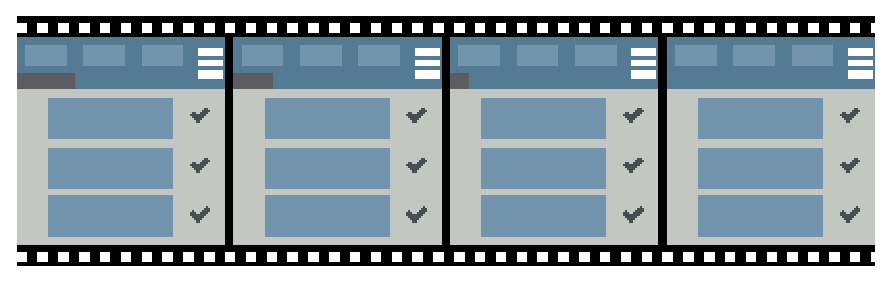
\includegraphics[width=\figscale\textwidth]{pictures/line1OutroFig}
\caption{The \hs{line1Out} animation.}
\label{fig:basic1_1}
\end{subfigure}

\begin{subfigure}[h]{\textwidth}
\centering
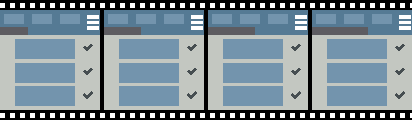
\includegraphics[width=\figscale\textwidth]{pictures/line2IntroFig}
\caption{The \hs{line2In} animation.}
\label{fig:basic1_2}
\end{subfigure}

\begin{subfigure}[h]{\textwidth}
\centering
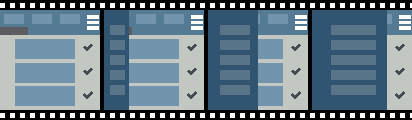
\includegraphics[width=\figscale\textwidth]{pictures/menuSlideInFig}
\caption{The \hs{menuSlideIn} animation.}
\label{fig:basic2_1}
\end{subfigure}

\begin{subfigure}[h]{\textwidth}
\centering
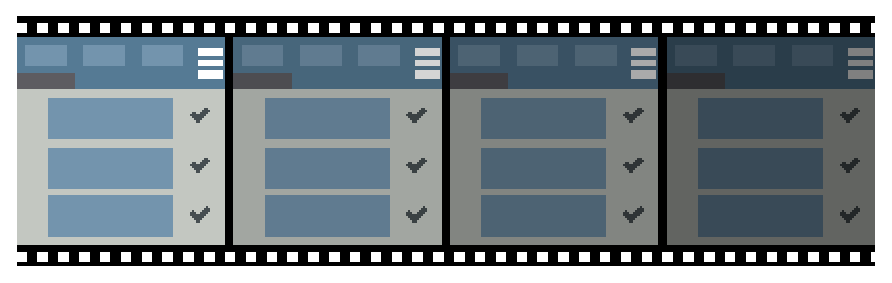
\includegraphics[width=\figscale\textwidth]{pictures/appFadeOutFig}
\caption{The \hs{appFadeOut} animation.}
\label{fig:basic2_2}
\end{subfigure}

\caption{Basic \hs{linearTo} animations.}
\label{fig:basic}
\end{figure}

\subsubsection{Composed Animations}

A composed animation combines several other animations into one new animation. We can do this either in \emph{sequence} or in \emph{parallel}.

We create the \hs{selectBtn2} animation by combining the \hs{line1Out} and \hs{line2In} animations with \hs{sequential}. This constructs a new animation which first plays \hs{line1Out}, and once it is finished plays \hs{line2In}.

\begin{spec}
selectBtn2Anim = line1Out `sequential` line2In
\end{spec}

To obtain the \hs{menuIntro} animation, we combine both the \hs{menuSlideIn} and \hs{appFadeOut} animations with \hs{parallel}. This constructs a new animation which plays both the \hs{menuSlideIn} and \hs{appFadeOut} animations at the same time.

\begin{spec}
menuIntro = menuSlideIn `parallel` appFadeOut
\end{spec}

Both of these animations are shown visually in Figure~\ref{fig:composed}.

\begin{figure}[!htbp]
\centering

\begin{subfigure}[h]{\textwidth}
\centering
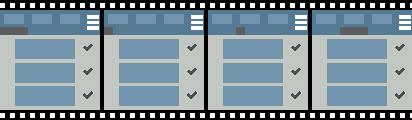
\includegraphics[width=\figscale\textwidth]{pictures/selectBtn2AnimFig}
\caption{The \hs{selectBtn2} animation.}
\label{fig:composed1}
\end{subfigure}

\begin{subfigure}[h]{\textwidth}
\centering
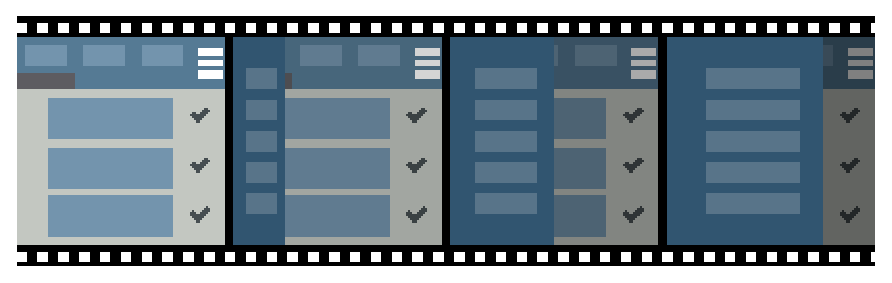
\includegraphics[width=\figscale\textwidth]{pictures/menuIntroFig}
\caption{The \hs{menuIntro} animation.}
\label{fig:composed2}
\end{subfigure}

\caption{All of the defined composed animations.}
\label{fig:composed}
\end{figure}
